\documentclass[noinstructornotes]{ximera}
%handout:  for handout version with no solutions or instructor notes
%handout,instructornotes:  for instructor version with just problems and notes, no solutions
%noinstructornotes:  shows only problem and solutions

%% handout
%% space
%% newpage
%% numbers
%% nooutcomes

%I added the commands here so that I would't have to keep looking them up
%\newcommand{\RR}{\mathbb R}
%\renewcommand{\d}{\,d}
%\newcommand{\dd}[2][]{\frac{d #1}{d #2}}
%\renewcommand{\l}{\ell}
%\newcommand{\ddx}{\frac{d}{dx}}
%\everymath{\displaystyle}
%\newcommand{\dfn}{\textbf}
%\newcommand{\eval}[1]{\bigg[ #1 \bigg]}

%\begin{image}
%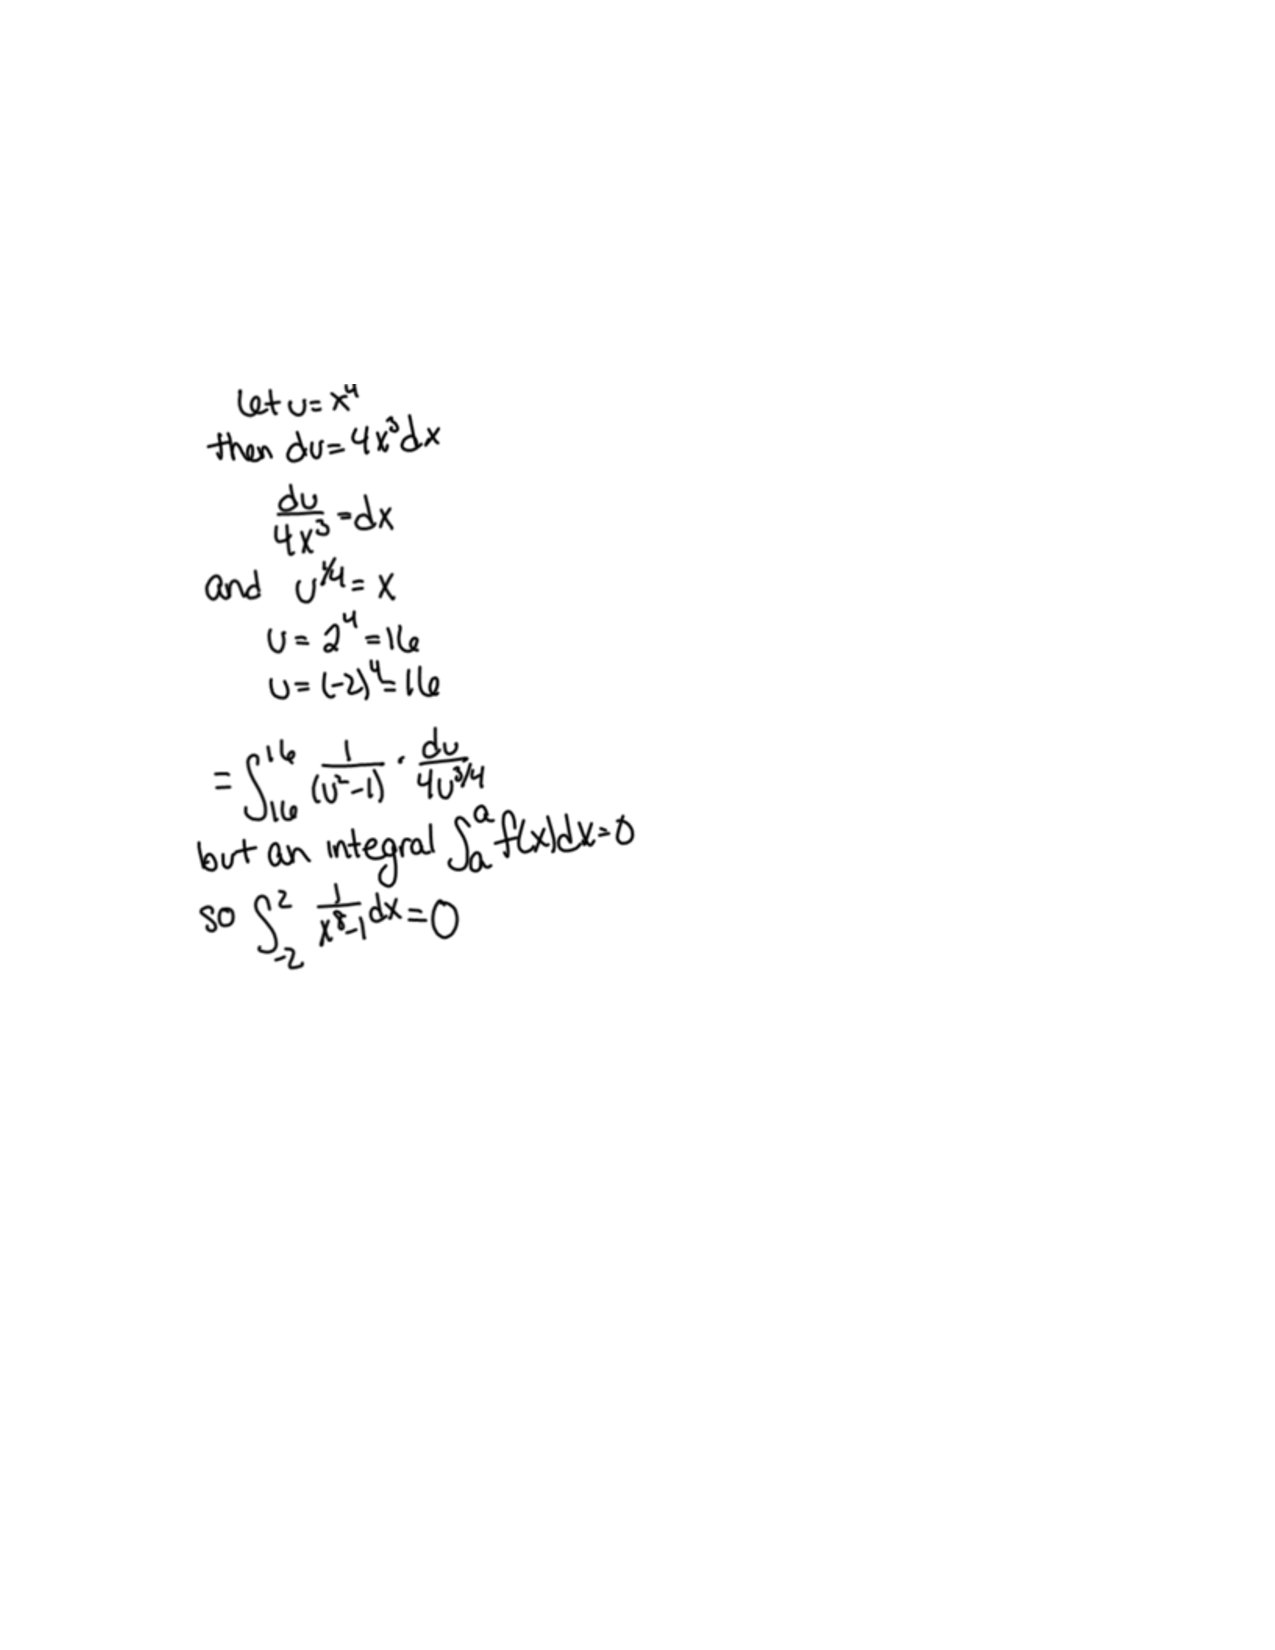
\includegraphics[trim= 170 420 250 180]{Figure1.pdf}
%\end{image}

%add a ``.'' below when used in a specific directory.
\newcommand{\RR}{\mathbb R}
\renewcommand{\d}{\,d}
\newcommand{\dd}[2][]{\frac{d #1}{d #2}}
\renewcommand{\l}{\ell}
\newcommand{\ddx}{\frac{d}{dx}}
\newcommand{\dfn}{\textbf}
\newcommand{\eval}[1]{\bigg[ #1 \bigg]}

\usepackage{multicol}

\renewenvironment{freeResponse}{
\ifhandout\setbox0\vbox\bgroup\else
\begin{trivlist}\item[\hskip \labelsep\bfseries Solution:\hspace{2ex}]
\fi}
{\ifhandout\egroup\else
\end{trivlist}
\fi} %% we can turn off input when making a master document

\title{Section 12.5: Lines and Curves in Space}  

\begin{document}
\begin{abstract}		\end{abstract}
\maketitle



\section{Warm up:}





\section{Group work:}

%problem 1
\begin{problem}
Find a vector-valued function for the line segment connecting the points $P = (-3,7,6)$ and $Q = (5,-4,7)$ in such a way that the value at $t=0$ is $P$ and the value at $t=1$ is $Q$.  
Also, find the point two-thirds of the way from $P$ to $Q$.
	\begin{freeResponse}
	The line segment $\vec{r}(t)$ from $P$ to $Q$ is 
		\begin{align*}
		\vec{r}(t) &= (1-t)P + tQ  \\
		&= (1-t) \langle -3,7,6 \rangle + t \langle 5,-4,7 \rangle  \\
		&= \boxed{\langle -3 + 8t, 7 - 11t, 6 + t \rangle \quad \text{for }0 \leq t \leq 1}.
		\end{align*}
	The point two-thirds of the way from $P$ to $Q$ is
		\begin{align*}
		\vec{r} \left( \frac{2}{3} \right)
		&= \left\langle -3 + 8 \left( \frac{2}{3} \right), 7 - 11\left( \frac{2}{3} \right), 6 + \frac{2}{3} \right\rangle  \\
		&= \boxed{\left\langle \frac{7}{3} , - \frac{1}{3}, \frac{20}{3} \right\rangle}
		\end{align*}
	\end{freeResponse}
	
\begin{instructorNotes}
A common mistake is to forget the domain of $t$. 
\end{instructorNotes}
\end{problem}


%problem 2
\begin{problem}
Find a vector-valued function for the line through the point $(1,-2,3)$ that is perpendicular to the lines
	\[
	\vec{r}_1(t) = \langle 7,8,-2 \rangle + t \langle 3,5,7 \rangle 
	\quad \text{and} \quad 
	\vec{r}_2(s) = \langle 4,-3,-7 \rangle + s \langle 4,9,-1 \rangle
	\]
	\begin{freeResponse}
	Let $\vec{v}_1 = \langle 3,5,7 \rangle$ and $\vec{v}_2 = \langle 4,9,-1 \rangle$.
	Then $\vec{v}_1$ is parallel to the line $\vec{r}_1$, and similarly for $\vec{v}_2$ and $\vec{r}_2$.  
	So a vector perpendicular to both of the lines $\vec{r}_1$ and $\vec{r}_2$ is
		\begin{align*}
		\vec{n} = \vec{v}_1 \times \vec{v}_2  
		&= \begin{vmatrix}
		\hat{\imath}	&	\hat{\jmath}	&	\hat{k}	\\
		3		&	5		&	7		\\
		4		&	9		&	-1		\\
		\end{vmatrix}  \\
		&= (-5-63)\hat{\imath} - (-3-28)\hat{\jmath} + (27-20)\hat{k}  \\
		&= \langle -68, 31, 7 \rangle.
		\end{align*}
	So the equation of the line through $(1,-2,3)$ and perpendicular to both $\vec{r}_1$ and $\vec{r}_2$ is
		\begin{align*}
		\vec{r}_3(t) &= \langle 1,-2,3 \rangle + t \langle -68,31,7 \rangle  \\
		&= \boxed{\langle 1-68t,-2+31t,3+7t \rangle \quad \text{for }-\infty < t < \infty}
		\end{align*}
	\end{freeResponse}
	
\end{problem}

\begin{instructorNotes}

\end{instructorNotes}















%problem 3
\begin{problem}
Show that the curve $\vec{r} = \langle t \cos t, t \sin t, t \rangle$ lies completely on the cone $z^2 = x^2 + y^2$.  
	\begin{freeResponse}
	We just need to check that the components of $\vec{r}$ satisfies the given equation.  
	So we compute
		\begin{align*}
		x^2 + y^2 &= (t \cos t)^2 + (t \sin t)^2  \\
		&= t^2 \cos^2 t + t^2 \sin^2 t  \\
		&= t^2 (\cos^2 t + \sin^2 t)  \\
		&= t^2  \\
		&= z^2.
		\end{align*}
	\end{freeResponse}

\end{problem}

\begin{instructorNotes}

\end{instructorNotes}




 
 






		












	
	
	
	
	
	
	
	
	

	










								
				
				
	














\end{document} 


















